\documentclass[a4paper]{article}
\usepackage[pdftex]{hyperref}
\usepackage[latin1]{inputenc}
\usepackage[english]{babel}
\usepackage{a4wide}
\usepackage{amsmath}
\usepackage{amssymb}
\usepackage{algorithmic}
\usepackage{algorithm}
\usepackage{ifthen}
\usepackage{listings}
% move the asterisk at the right position
\lstset{basicstyle=\ttfamily,tabsize=4,literate={*}{${}^*{}$}1}
%\lstset{language=C,basicstyle=\ttfamily}
\usepackage{moreverb}
\usepackage{palatino}
\usepackage{multicol}
\usepackage{tabularx}
\usepackage{comment}
\usepackage{verbatim}
\usepackage{color}

% Because of an error on line 41 I added this
\usepackage{graphicx}

% Used for drawing DFAs and NFAs
\usepackage{tikz}
\usetikzlibrary{automata, positioning}

% Defined checkmark sign
\def\checkmark{\tikz\fill[scale=0.4](0,.35) -- (.25,0) -- (1,.7) -- (.25,.15) -- cycle;}

% Table coloring
\usepackage{color, colortbl}
\usepackage[first=0,last=9]{lcg}

% Tab
\newcommand\tab[1][1.15cm]{\hspace*{#1}}

%% pdflatex?
\newif\ifpdf
\ifx\pdfoutput\undefined
\pdffalse % we are not running PDFLaTeX
\else
\pdfoutput=1 % we are running PDFLaTeX
\pdftrue
\fi
%\ifpdf
%\usepackage[pdftex]{graphicx}
%\else
%\usepackage{graphicx}
%\fi
\ifpdf
\DeclareGraphicsExtensions{.pdf, .jpg}
\else
\DeclareGraphicsExtensions{.eps, .jpg}
\fi

\parindent=0cm
\parskip=0cm

\setlength{\columnseprule}{0.4pt}
\addtolength{\columnsep}{2pt}

\addtolength{\textheight}{5.5cm}
\addtolength{\topmargin}{-26mm}
\pagestyle{empty}

%%
%% Sheet setup
%% 
\newcommand{\coursename}{Computability and Complexity}
\newcommand{\courseno}{CO21-320352}
 
\newcommand{\sheettitle}{Homework}
\newcommand{\mytitle}{}
\newcommand{\mytoday}{February 12th, 2019}

% Current Assignment number
\newcounter{assignmentno}
\setcounter{assignmentno}{1}

% Current Problem number, should always start at 1
\newcounter{problemno}
\setcounter{problemno}{1}

%%
%% problem and bonus environment
%%
\newcounter{probcalc}
\newcommand{\exercise}[2]{
  \pagebreak[2]
  \setcounter{probcalc}{#2}
  ~\\
  {\large \textbf{Exercise \arabic{problemno}} \hspace{0.2cm}\textit{#1}} \refstepcounter{problemno}\vspace{2pt}\\}

\newcommand{\bonus}[2]{
  \pagebreak[2]
  \setcounter{probcalc}{#2}
  ~\\
  {\large \textbf{Bonus Problem \textcolor{blue}{\arabic{assignmentno}}.\textcolor{blue}{\arabic{problemno}}} \hspace{0.2cm}\textit{#1}} \refstepcounter{problemno}\vspace{2pt}\\}

%% some counters  
\newcommand{\assignment}{\arabic{assignmentno}}

%% solution  
\newcommand{\solution}{\pagebreak[2]{\bf Solution:}\\}

%% Hyperref Setup
\hypersetup{pdftitle={Homework \assignment},
  pdfsubject={\coursename},
  pdfauthor={},
  pdfcreator={},
  pdfkeywords={Computability and Complexity},
  %  pdfpagemode={FullScreen},
  %colorlinks=true,
  %bookmarks=true,
  %hyperindex=true,
  bookmarksopen=false,
  bookmarksnumbered=true,
  breaklinks=true,
  %urlcolor=darkblue
  urlbordercolor={0 0 0.7}
}

\begin{document}
\coursename \hfill Course: \courseno\\
Jacobs University Bremen \hfill \mytoday\\
Dragi Kamov and Dushan Terzikj\hfill
\vspace*{0.3cm}\\
\begin{center}
{\Large \sheettitle{} \assignment\\}
\end{center}

\exercise{}{0}
\solution
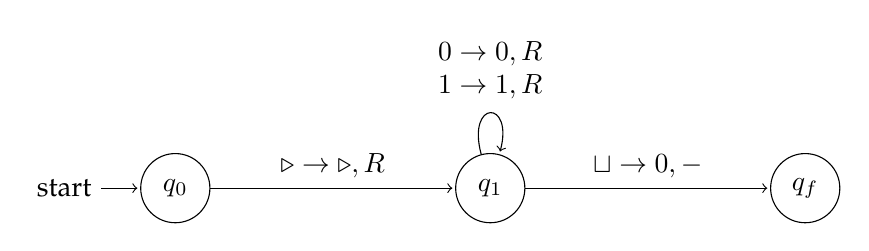
\begin{tikzpicture}[shorten >=1pt,node distance=4cm,on grid,auto]
   \node[state,initial] (0) {$ q_0 $};
   \node[state] (1) [right=of 0] {$ q_1 $};
   \node[state] (2) [right=of 1] {$ q_f $};
   \path[->]
    (0) edge                    node {$ \triangleright \rightarrow \triangleright, R $} (1)
    (1) edge                    node {$ \sqcup \rightarrow 0, - $} (2)
    (1) edge [loop above]       node {$ \begin{matrix}0 \rightarrow 0, R \\ 1 \rightarrow 1, R \end{matrix} $} (1);
\end{tikzpicture}
\begin{center}
    \begin{tabular}{|c|c|c|} \hline
        p $ \in $ K & $ \sigma \in \Sigma $ & $ \delta $(p, $ \sigma $)  \\ \hline
        $ q_0 $ & $ \triangleright $ & ($ q_1 $, $ \triangleright $, $ \rightarrow $) \\ \hline
        $ q_1 $ & 0 & ($ q_1 $, 0, $ \rightarrow $) \\ \hline
        $ q_1 $ & 1 & ($ q_1 $, 1, $ \rightarrow $) \\ \hline
        $ q_1 $ & $ \sqcup $ & ($ q_f $, 0, -) \\ \hline
    \end{tabular}
\end{center}
 
\exercise{}{0}
\solution
According to the lecture notes, this is the definition about an ordinary Turing machine: \\

\textit{\textbf{Definition 3.1:} A Turing machine is a structure M = (K, $ \Sigma $, $ \delta $, s), where K is a finite set of states, s $ \in $ K is the initial state, the alphabet $ \Sigma $ is a set of (tape) symbols, and where K and $ \Sigma $ are disjoint. We assume that $ \Sigma $ always contains the special symbols $ \sqcup $ and $ \triangleright $, the blank and the first symbol. Finally, $ \delta $ is a transition function, where \\
$ \delta $: K $\times $ $ \Sigma $ $ \rightarrow $ (K $ \cup $ \{h, "yes", "no"\}) $ \times $ $ \Sigma $ $ \times $ \{$ \leftarrow $, $ \rightarrow $, - \}. \\
We assume that h (the halting state), "yes" (the accepting state), "no" (the rejecting state), and the cursor directions $ \leftarrow $ for "left", $ \rightarrow $ for "right" and - for "stay", are extra symbols not in K $ \cup $ $ \Sigma $.} \\

And if one were to admit TMs with countably many states that would look like this: \\
An infinite Turing machine is a quadruple M = (K; $ \Sigma $; $ \delta $; s), where $ \Sigma $ and s are exactly as an ordinary Turing machine, but the set K must contain infinite states. $ \delta $ is a transition function that must reflect the complexities of infinite states. Intuitively, $ \delta $ decides the next state as before, but also contains infinite actions (steps). Nevertheless, the final states are unique, that is there should be only one h (the halting state), "yes" (the accepting state) and "no" (the rejecting state) in M. \\

So answering the question from the problem sheet, having countably infinitely many states doesn't open doors to solving problems that ordinary TM couldn't, but it might compute functions much faster since it has more states.

\end{document}